\documentclass[12pt]{article}
	
\usepackage[margin=1in]{geometry}		% For setting margins
\usepackage{amsmath}				% For Math
\usepackage{fancyhdr}				% For fancy header/footer
\usepackage{graphicx}				% For including figure/image
\usepackage{cancel}					% To use the slash to cancel out stuff in work

%%%%%%%%%%%%%%%%%%%%%%
% Set up fancy header/footer
\pagestyle{fancy}
\fancyhead[LO,L]{Kate O'Neill - 21365768}
\fancyhead[CO,C]{CSU11031 - Electronics Assignment 1}
\fancyhead[RO,R]{\today}
\fancyfoot[LO,L]{}
\fancyfoot[CO,C]{\thepage}
\fancyfoot[RO,R]{}
\renewcommand{\headrulewidth}{0.4pt}
\renewcommand{\footrulewidth}{0.4pt}
%%%%%%%%%%%%%%%%%%%%%%

\begin{document}
\noindent 1.) Connect up online the circuit below using Multisim from National Instruments:\\
Place voltmeters at each node of the circuit and ammeters at each branch.\\ Run the simulation.\\
\\
\begin{figure}[!h] 
	\begin{centering}
		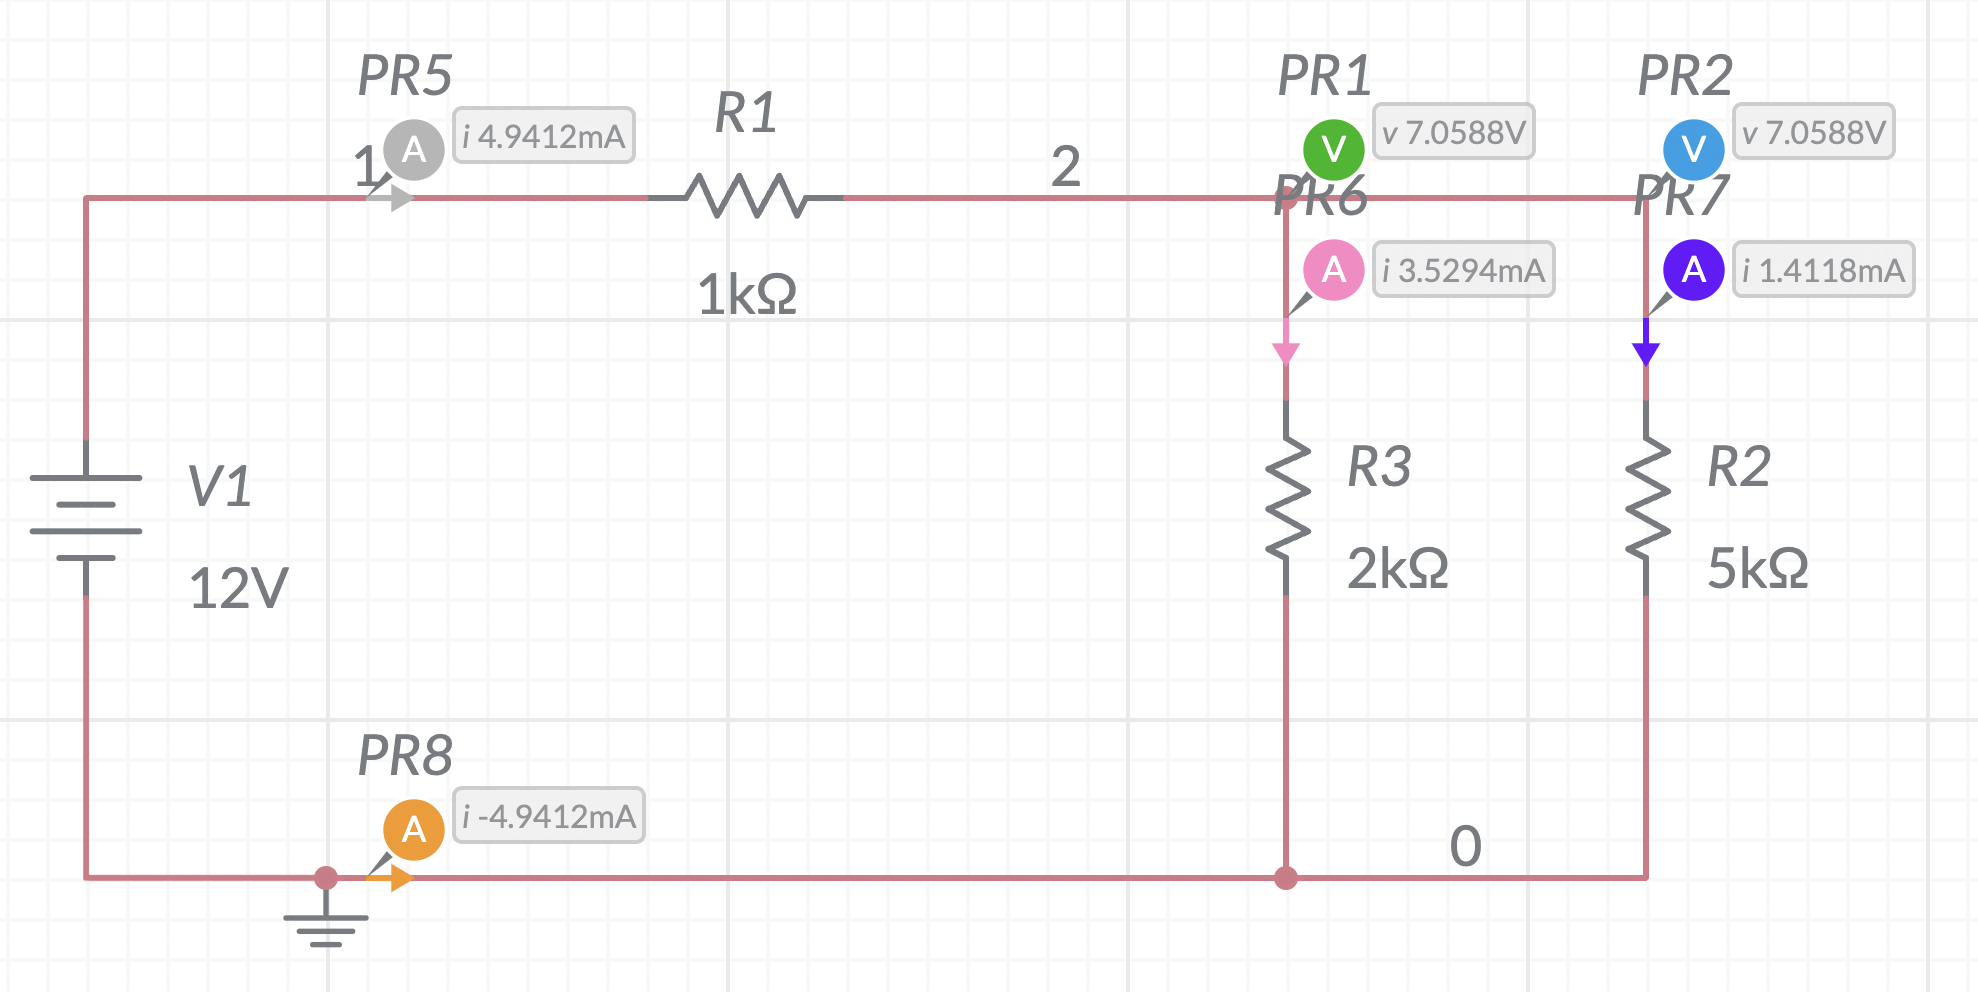
\includegraphics[keepaspectratio = true, width = 5in]{Q1(i).png}
	\end{centering}
\end{figure}\\
\noindent (i) Verify by calculation that each of the voltage and current values shown are correct. Use the Voltage Divider rule to verify the voltage at Node 2.\\

\noindent Beginning with parallel resistors R2 and R3,\\
\[\frac{1}{R_T} = \frac{1}{R_1} + \frac{1}{R_2} + ... + \frac{1}{R_n}\]
\[\frac{1}{R_T} = \frac{1}{2000} + \frac{1}{5000} = \frac{7}{10000}\]
\[R_T = \frac{10000}{7}\Omega\]\\
Now we can add all of the resistors together as if they are in series.\\
\[R_{Total} = R_1 + R_2 + ... + R_n\]
\[R_{Total} = 1000 + \frac{10000}{7} = \frac{17000}{7}\Omega\]\\
Having found the total resistance, we can now calculate the total current running through the circuit using Ohm's Law.\\
\[V = IR\]
\[12 = \frac{17000}{7}I\]
\(\)\[I = \frac{21}{4250}A = 4.9412mA\]\\
As we can see, this value is consistent with what is shown on the diagram above by ammeter PR5.\\
The current flowing through PR8 is also 4.9412mA, however it is flowing in the opposite direction hence the negative value.\\
Now that we have both the resistance and the current, we can use these to calculate the voltage across the voltmeters.\\
To find the voltage drop after R1,\\
\[V = IR\]
\[V = (4.9412 \times 10^{-3}) \times 1000\]
\[V = 4.9412V\]\\
The voltage drops as it leaves R1, meaning that in node 2 the voltage is\\
\[12 - 4.9412 = 7.0588V\]\\
This matches the information provided by PR1.\\
Voltage in parallel is given by\\
\[V_1 = V_2 = V_3 = ... = V_n\]\\
Therefore,\\
\[V_{PR1} = V_{PR2} = 7.0588V\]\\
Now we have enough information to verify ammeters PR6 and PR7.\\
Starting with PR6,\\
Again using Ohm's Law,
\[V = IR\]
\[7.0588 = 2000I\]
\[I = 7.0588 / 2000\]
\[I = 3.5294 \times 10^{-3}\]
\[I = 3.5294mA\]\\
Moving onto PR7,\\
\[7.0588 = 5000I\]
\[I = 7.0588 / 5000\]
\[I = 1.41176 \times 10^{-3}A\]
\[I = 1.41176mA\]\\
To verify voltage at Node 2, we shall be using the voltage divider rule.\\
Resistors R2 and R3 are connected in parallel.
\[\frac{1}{R_T} = \frac{1}{2000} + \frac{1}{5000} = \frac{7}{10000}\]
\[R_T = \frac{10000}{7}\Omega\]\\
We can now consider R2 and R3 as a single resistor in series with R1.\\
\[R_{Total} = 1000 + \frac{10000}{7} = \frac{1700}{7}\]\\
Using the voltage divider rule,
\[V_{Node 2} = V_{in}(\frac{R_T}{R_{Total}}) = \frac{120}{7}V\]\\
\\
(ii) Verify by calculation Kirchhoff's Current Law for the circuit. Compare with the results given by the simulator.\\
\\
\textit{Kirchoff’s Current Law (KCL) states that the algebraic sum of electrical currents at any node in an electrical circuit is equal to zero at every instant in time.}\\
To verify this, I will place additional ammeters on the diagram in order to measure the current flowing out of each node.\\
\\
\begin{figure}[!h] 
	\begin{centering}
		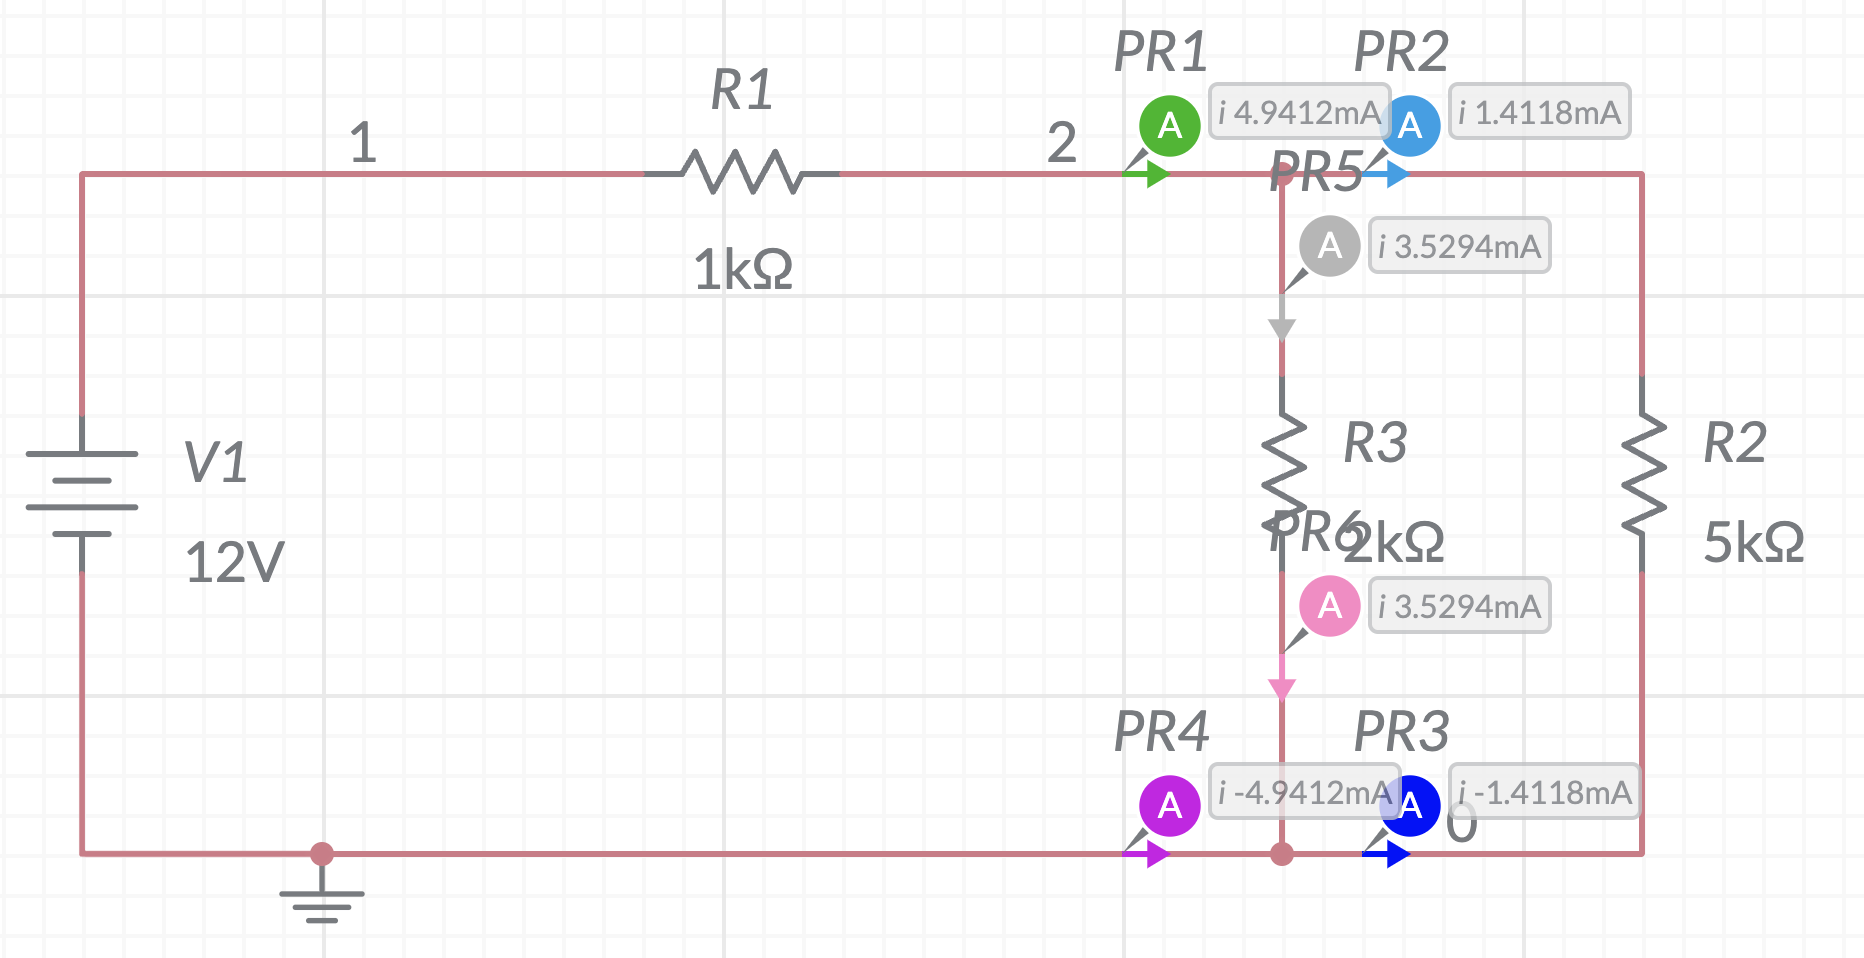
\includegraphics[keepaspectratio = true, width = 5in]{Q1(ii).png}
	\end{centering}
\end{figure}\\
\noindent By adding the charges going through R2 and R3, we can verify Kirchhoff's Current Law.\\
Beginning with Node 2,\\
\[PR1 - PR2 - PR5 = 0\]
\[4.9412 - 1.4118 - 3.5294 = 0\]\\
\\
Continuing with Node 3,\\
\[PR3 - PR4 - PR6 = 0\]
\[-1.4118 - (-4.9412) - 3.5294 = 0\]\\
\\
The results of these calculations verify Kirchhoff's Current Law as the current entering each node is equal the the current exiting each node.\\
\\
(iii) Verify by calculation Kirchhoff's Voltage Law for the circuit. Compare with the results given by the simulator.\\
\textit{Kirchoff’s Voltage Law (KVL) states that the algebraic sum of branch voltages around any loop in an electrical circuit is equal to zero at every instant in time.}\\
To verify this, I will place voltmeters at every resistor on the diagram.\\
\begin{figure}[!h] 
	\begin{centering}
		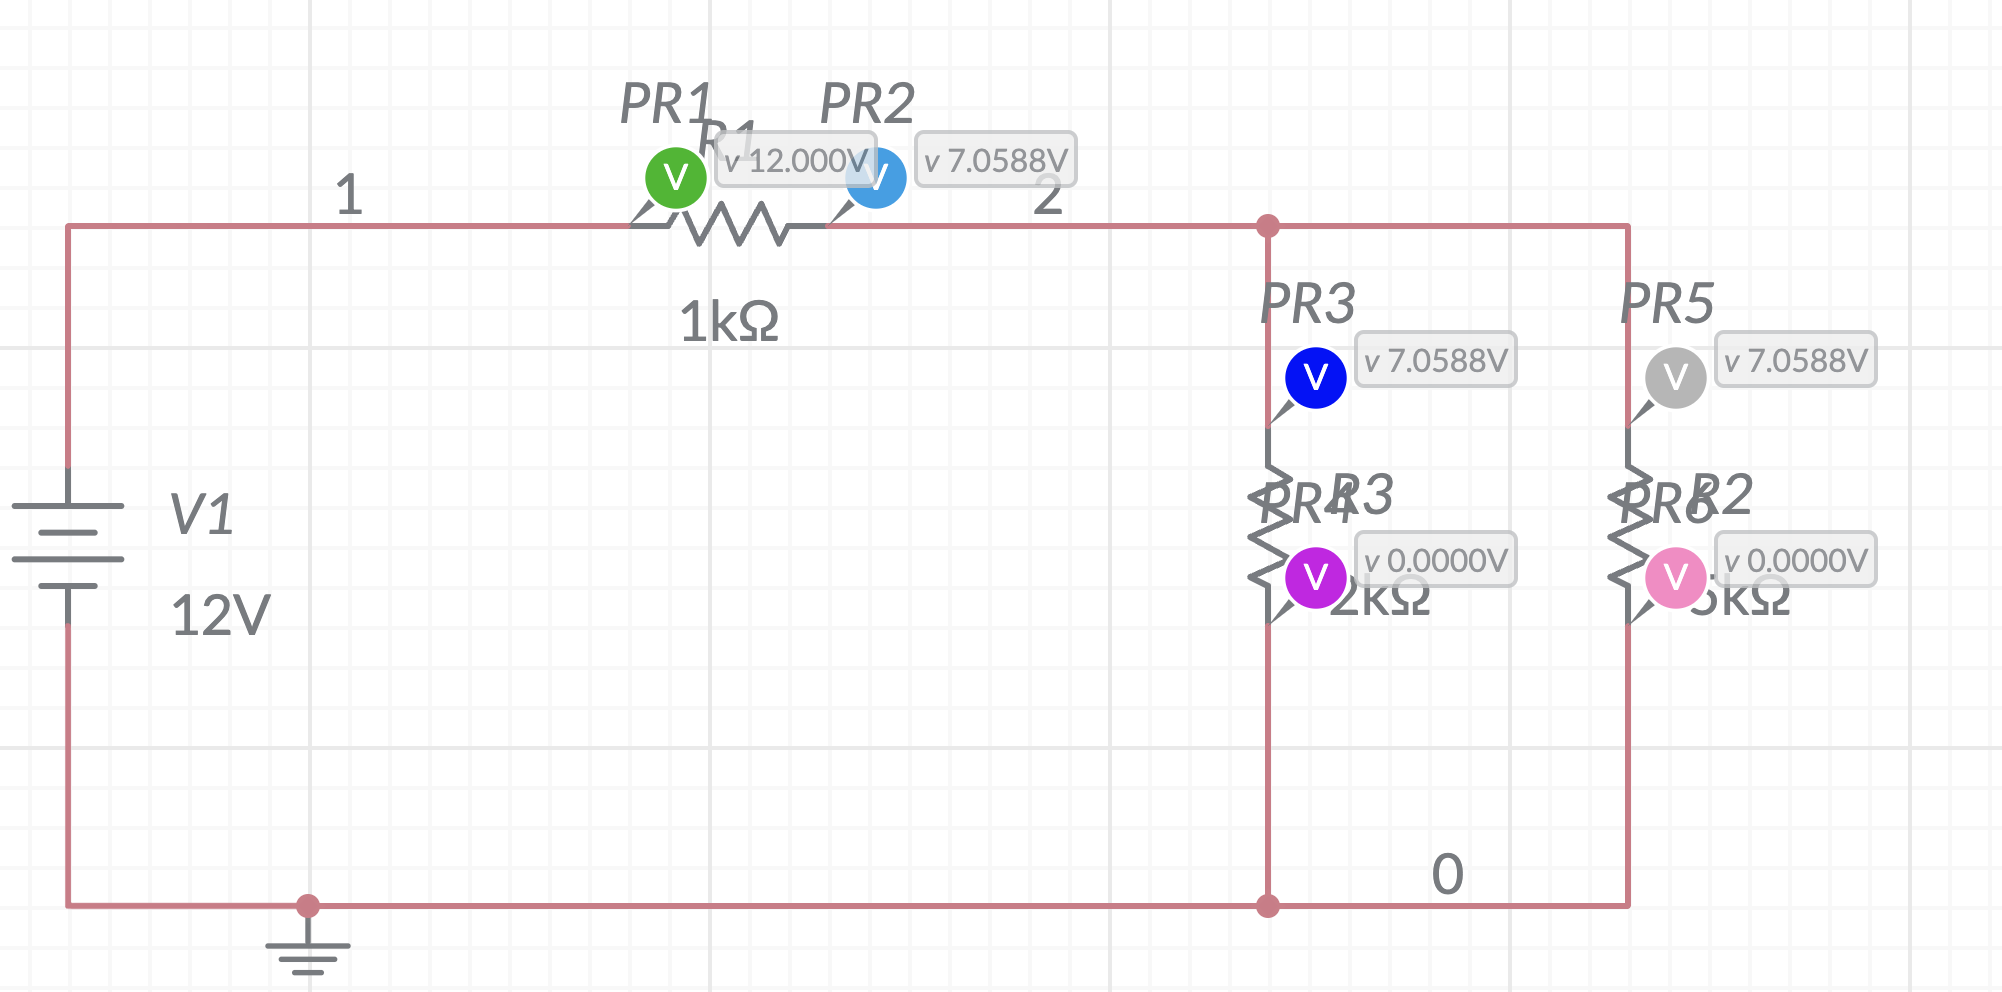
\includegraphics[keepaspectratio = true, width = 5in]{Q1(iii).png}
	\end{centering}
\end{figure}\\
Starting with the loop containing R1 and R3,\\
\[V_{Supply} - V_{R1} - V_{R3} = 0\]
\[12 - 4.9412 - 7.0588 = 0\]\\
\\
The voltmeters in the diagram show the current dropping 4.9412V after passing through R1, and dropping 7.0588V after passing through R3. After R3, the voltmeter reads 0.0000V and thus verifies Kirchhoff's Voltage Law.\\
\\
Then the loop containing R1 and R2,\\
\[V_{Supply} - V_{R1} - V_{R2} = 0\]
\[12 - 4.9412 - 7.0588 = 0\]\\
\\
The voltmeters in the diagram show the current dropping 4.9412V after passing through R1, and dropping 7.0588V after passing through R2. After R2, the voltmeter reads 0.0000V and thus verifies Kirchhoff's Voltage Law.\\
\\
(iv) Replace the battery with a 12V (peak) ac source, run the simulation, observe Grapher and explain your results.\\
\begin{figure}[!h] 
	\begin{centering}
		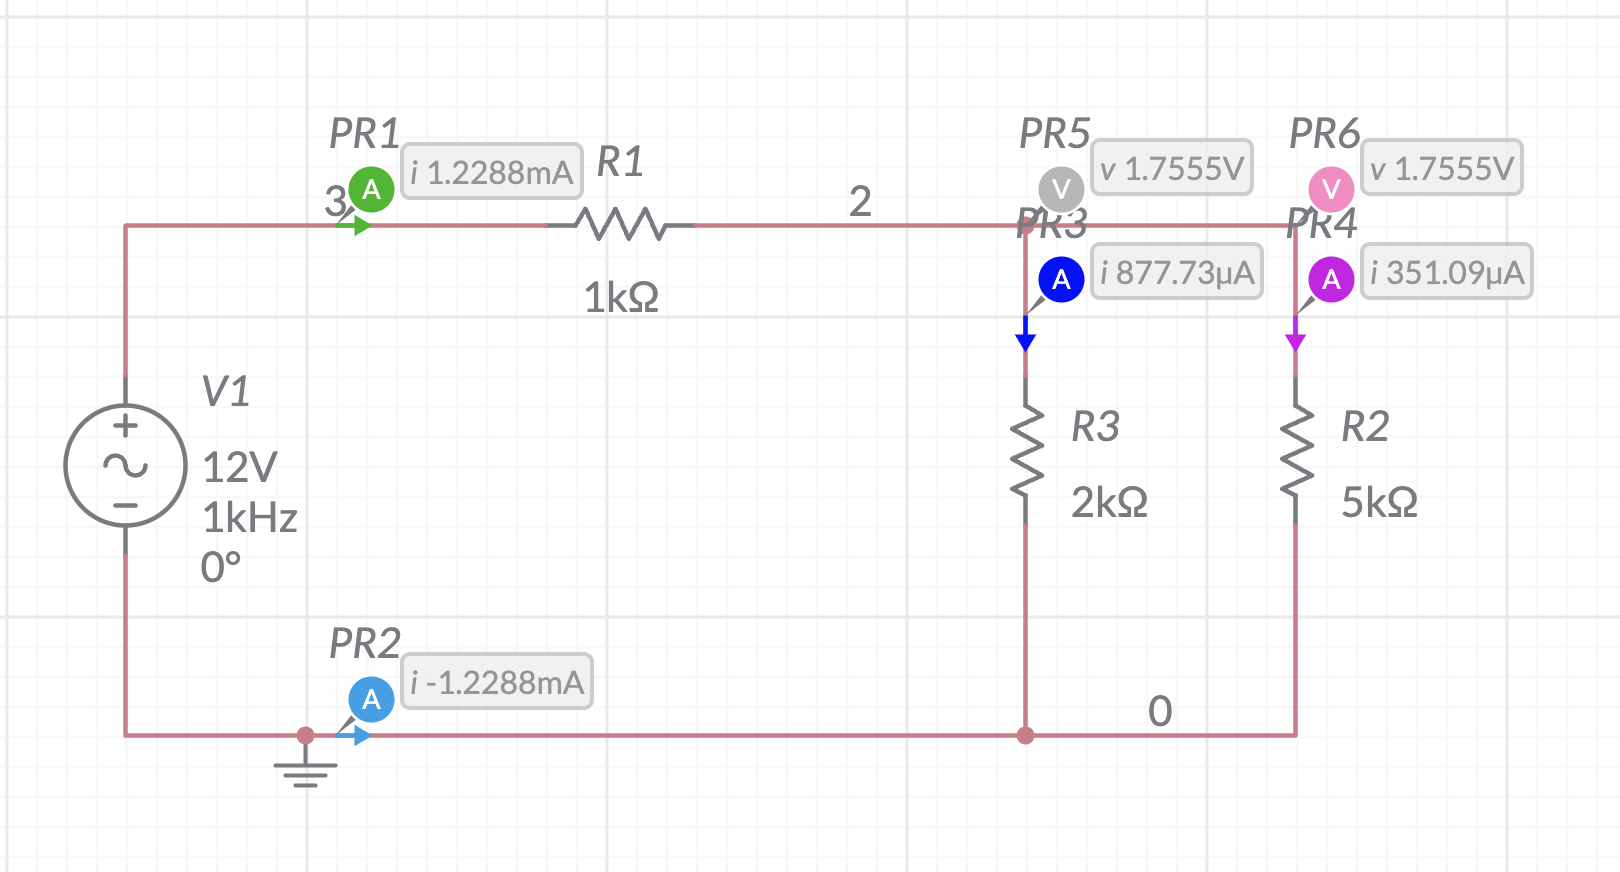
\includegraphics[keepaspectratio = true, width = 5in]{Q1(iv).png}
	\end{centering}
\end{figure}\\
\begin{figure}[!h] 
	\begin{centering}
		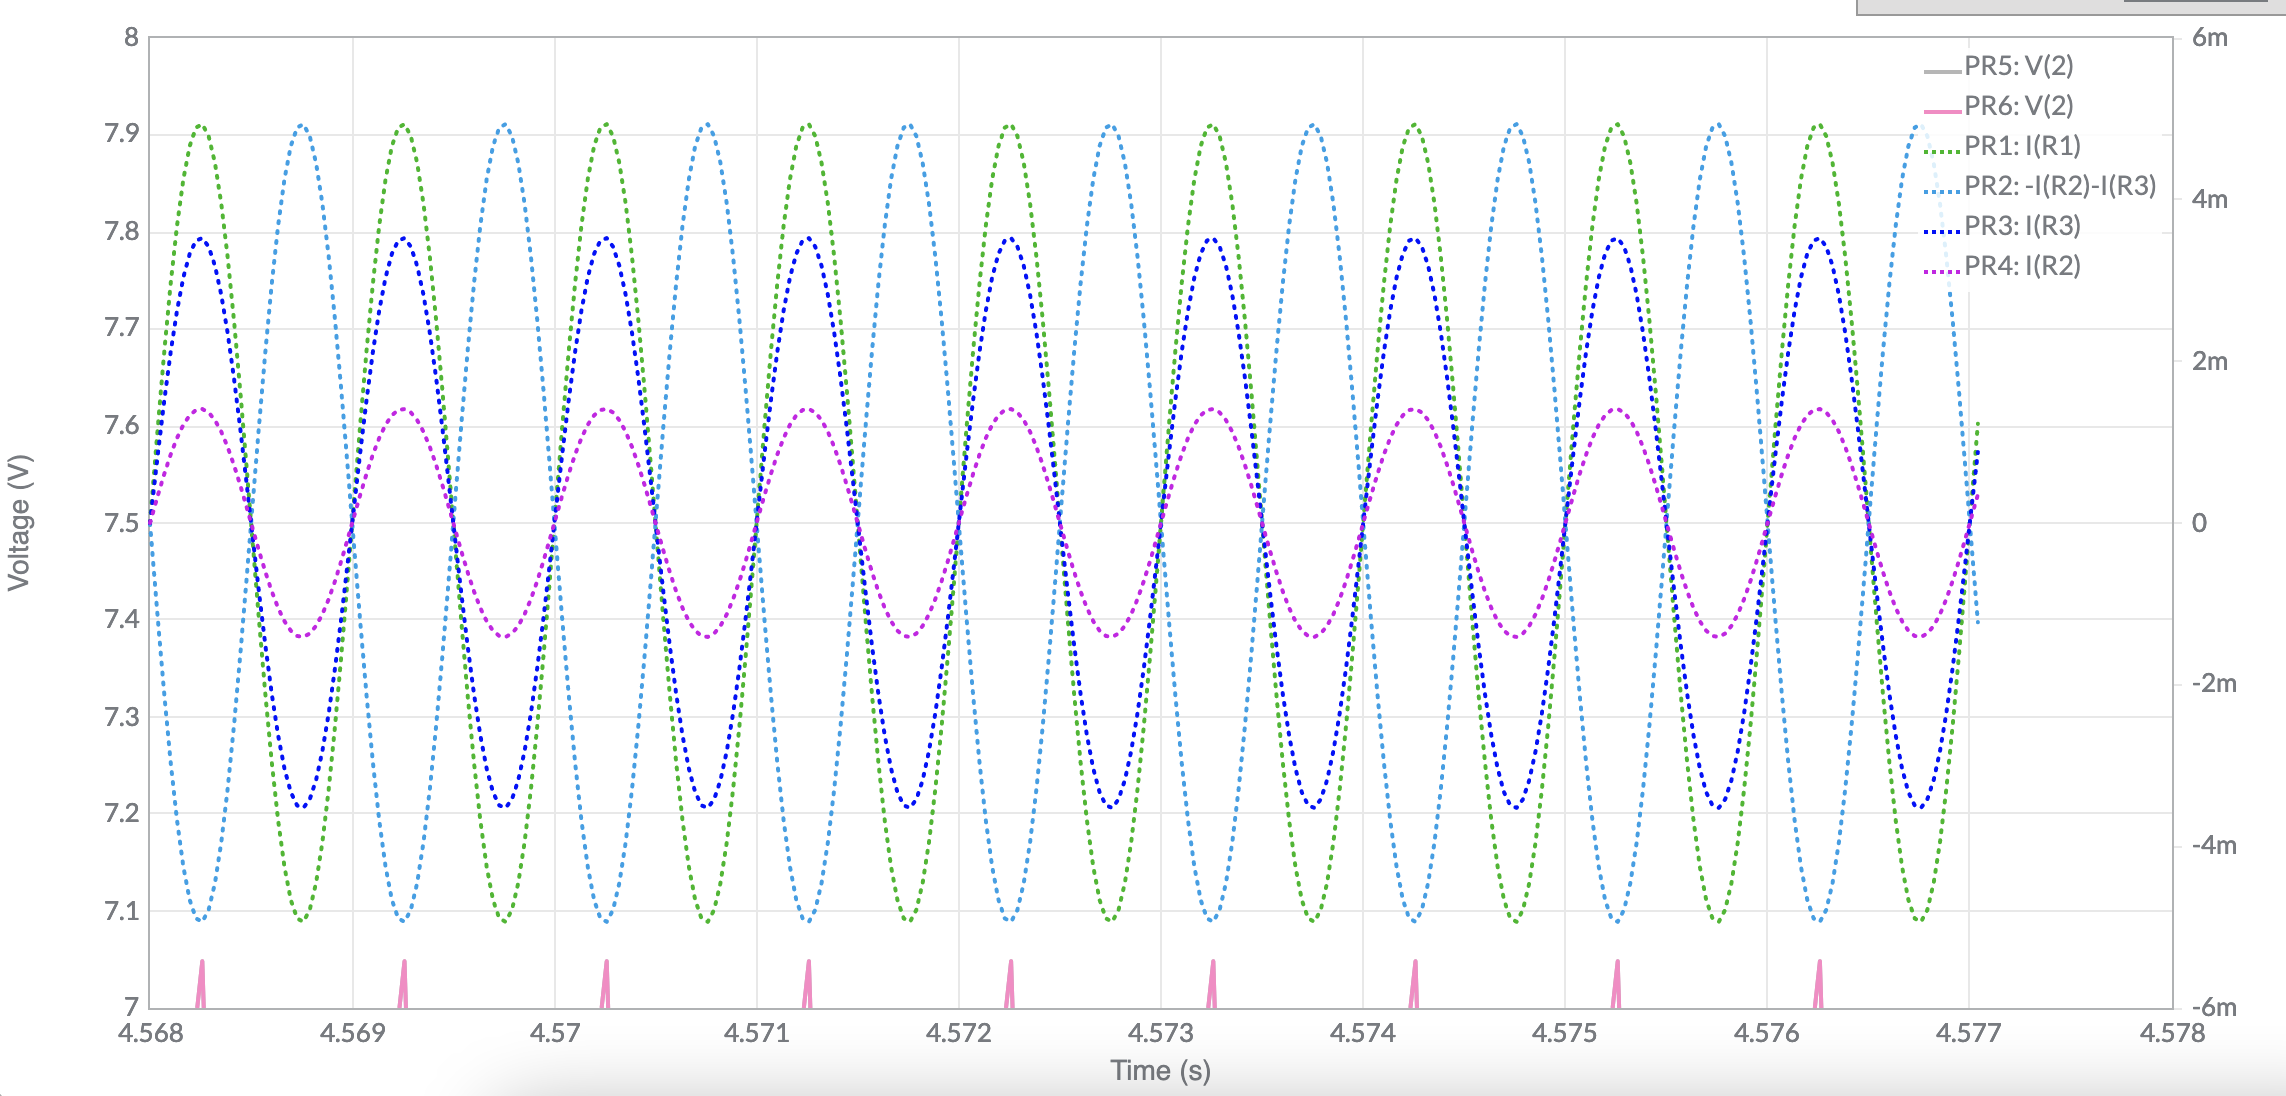
\includegraphics[keepaspectratio = true, width = 3in]{Q1(iv(i)).png}
	\end{centering}
\end{figure}\\
\\
\noindent The A.C. Power source creates a fluctuating graph, different from the straight line graph that would be observed with a D.C. source. This is because the battery is an ideal power source and doesn't change.\\
\\
2.) Connect up the circuit below. You can assume the resistance of the lamp is about 10 Ohms. You should support your answers with calculations.\\
\\
\begin{figure}[!h] 
	\begin{centering}
		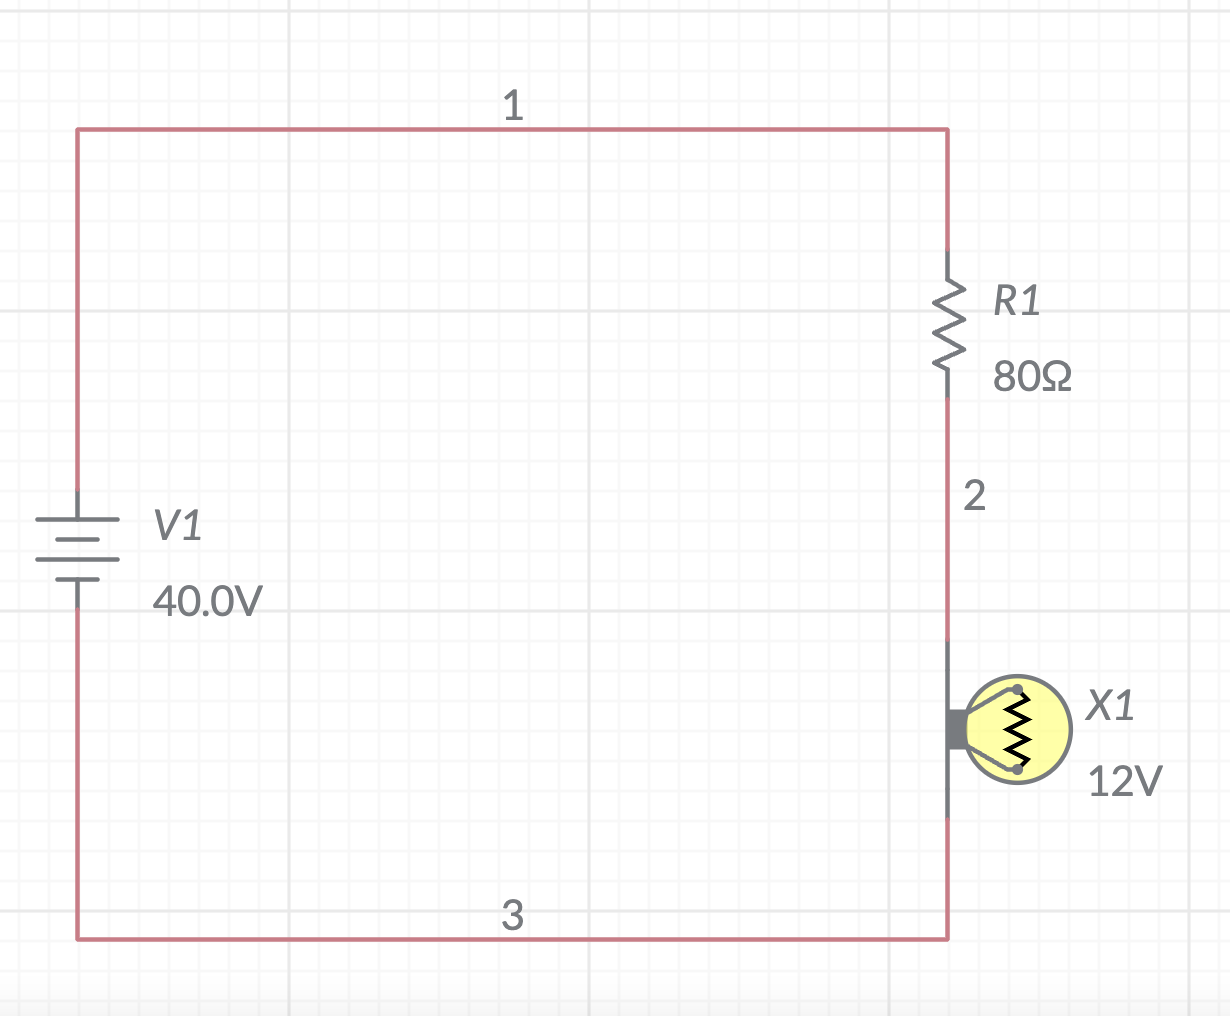
\includegraphics[keepaspectratio = true, width = 5in]{Q2(i).png}
	\end{centering}
\end{figure}\\
\noindent (i) Run the simulation. What do you observe?\\
\\
The lamp lights up when the simulation is run.\\
\\
As the resistors are in series, total resistance is given by,\\
\[R_{Total} = R_1 + R_2 + ... + R_n\]
\[R_{Total} = 80 + 10 = 90\Omega\]\\
We can now find the current flowing through this circuit using Ohm's Law.\\
\[V = IR\]
\[40 = 90I\]
\[I = \frac{4}{9}A = 0.4444A\]\\
Having found this information, we can now calculate the voltage across R1 and X1.\\
\\
Starting with R1,\\
\[V_{R1} = I_{R1}R_{R1}\]
\[V_{R1} = \frac{4}{9} \times 80 = \frac{320}{9}V = 35.5556V\]\\
\\
Moving onto X1,\\
\[V_{X1} = I_{X1}R_{X1}\]
\[V_{X1} = \frac{4}{9} \times 10 = \frac{40}{9}V = 4.4444V\]\\
We can see with these calculations that X1 only uses 4.4444V. The current drops by 35.5556V after R1 because of its high resistance.\\
\\
(ii) Replace R1 with a 1K resistor. What do you observe and why?\\
\\
\begin{figure}[!h] 
	\begin{centering}
		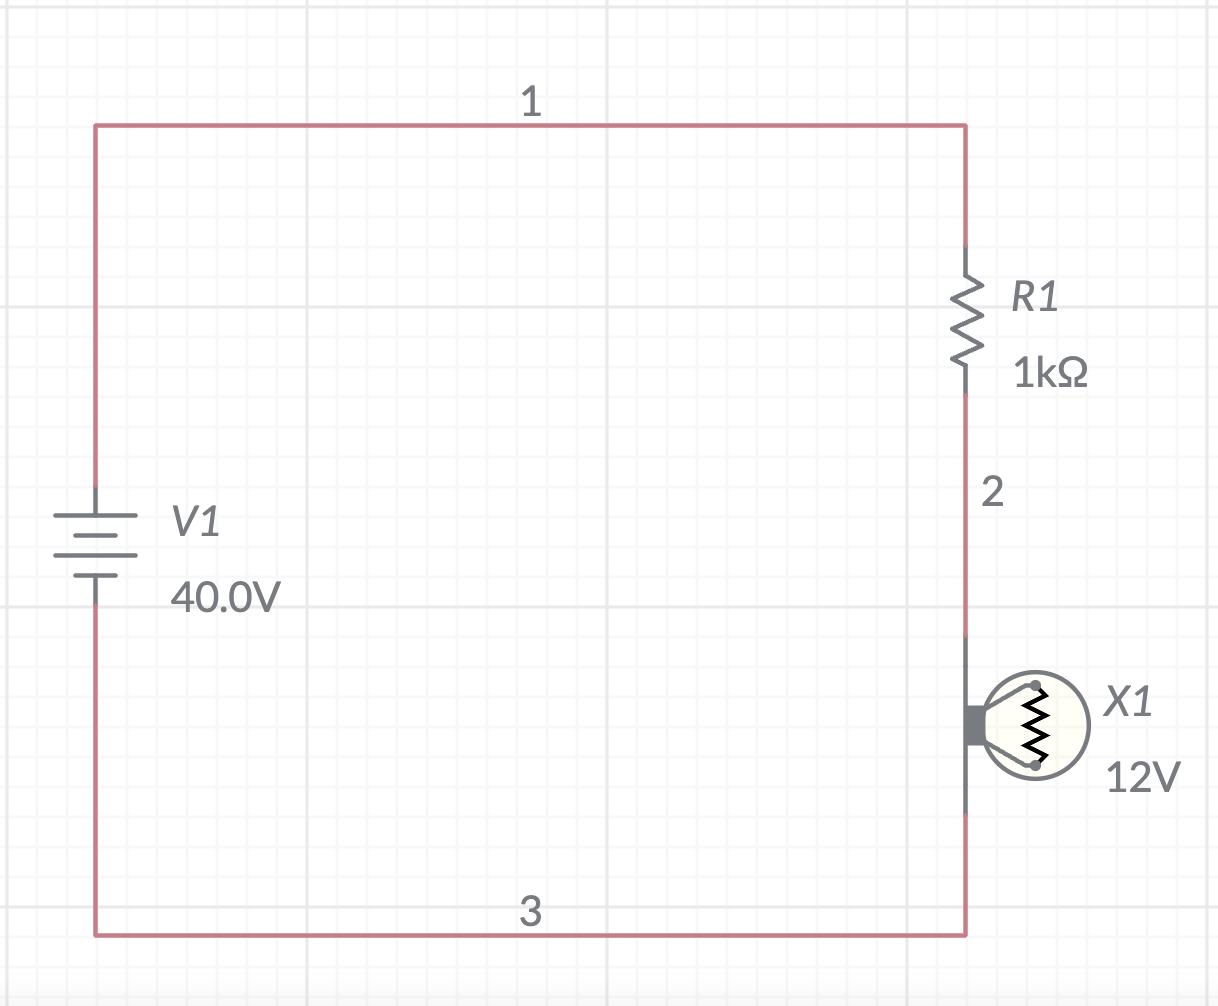
\includegraphics[keepaspectratio = true, width = 4in]{Q2(ii).png}
	\end{centering}
\end{figure}\\
After replacing R1 and running the simulation, we can see that the bulb does not turn on at all. From this, we can deduce that the higher the resistance of the resistor in series with a light bulb, the less energy received by the light bulb.\\
\\
As the resistors are in series, total resistance is given by,\\
\[R_{Total} = R_1 + R_2 + ... + R_n\]
\[R_{Total} = 1000 + 10 = 1010\Omega\]\\
We can now find the current flowing through this circuit using Ohm's Law.\\
\[V = IR\]
\[40 = 1010I\]
\[I = \frac{4}{101}A = 0.0396A\]\\
Having found this information, we can now calculate the voltage across R1 and X1.\\
\\
Starting with R1,\\
\[V_{R1} = I_{R1}R_{R1}\]
\[V_{R1} = \frac{4}{101} \times 1000 = \frac{4000}{101}V = 39.6039V\]\\
\\
Moving onto X1,\\
\[V_{X1} = I_{X1}R_{X1}\]
\[V_{X1} = \frac{4}{101} \times 10 = \frac{40}{101}V = 0.3960V\]\\
The calculations show that X1's input is extremely low, explaining why it appears to be off. This is because the voltage drops by 39.6039V as it passes through R1.\\
\\
(iii) With R1 at 80 Ohms, place a 1K resistor in parallel with the lamp. What do you observe and why?\\
\newpage
\begin{figure}[!h] 
	\begin{centering}
		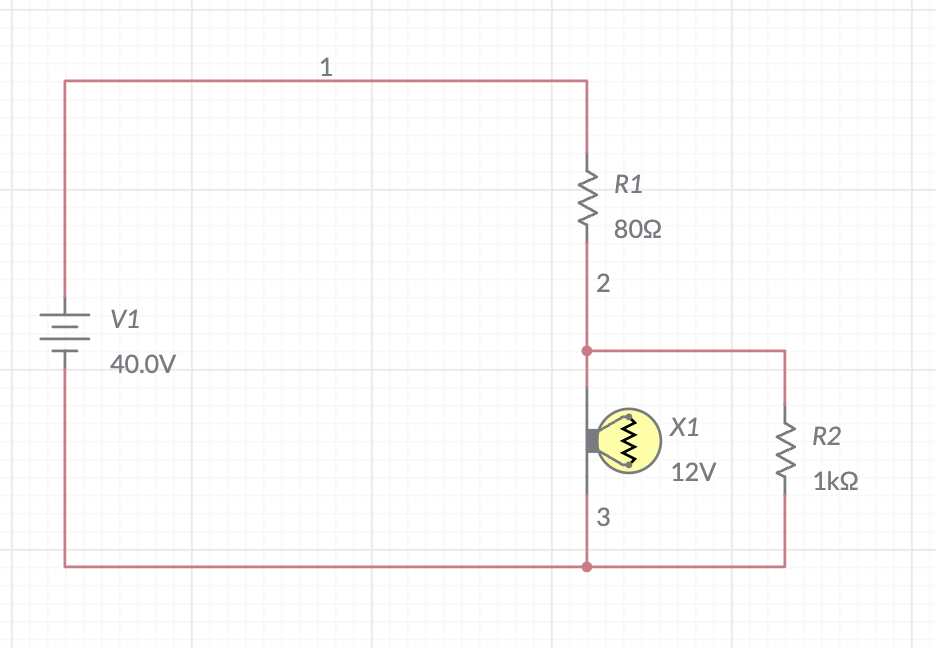
\includegraphics[keepaspectratio = true, width = 5in]{Q2(iii).png}
	\end{centering}
\end{figure}\\
\noindent It was observed that the brightness of X1 seems to stay the same as R2 is placed parallel to it.
\\
As X1 and R2 are parallel, we use the following formula to calculate their combined resistance.\\
\[\frac{1}{R_T} = \frac{1}{R_1} + \frac{1}{R_2} + ... + \frac{1}{R_n}\]
\[\frac{1}{R_T} = \frac{1}{10} + \frac{1}{1000} = \frac{101}{1000}\]
\[R_T = \frac{1000}{101}\Omega = 9.9009\Omega \]\\
Now we can treat all of our components as if they are in series.\\
\[R_{Total} = R_1 + R_2 + ... + R_n\]
\[R_{Total} = 80 + \frac{1000}{101} = \frac{9088}{101}\Omega = 89.9802\Omega\]\\
Using Ohm's Law, we can now find the current flowing through the circuit.\\
\[V = IR\]
\[40 = \frac{9080}{101}I\]
\[I = \frac{101}{227}A = 0.4449A\]\\
Using these values, we can now calculate the voltage drop after passing through each component.\\
\\
Starting with R1,\\
\[V_{R1} = I_{R1}R_{R1}\]
\[V_{R1} = \frac{101}{221} \times 80 = \frac{8080}{227}V = 35.5947V\]\\
As X1 and R2 are parallel to each other, their voltages are equal.\\
We can calculate the voltage drop across X1 and R2 like so\\
\[V_{in} = V_{R1} + V_{R2}\]
\[40 = \frac{8080}{227} + V_{R2}\]
\[V_{R2} = V_{X1} = 40 - \frac{8080}{227} = 4.4053V\]\\
These calculations show that the bulb is on because it has a higher input than in Q2(ii).\\
\\
(iv) Replace the parallel 1K resistor with a 10 Ohm resistor keeping R1 at 80 Ohms. What do you observe and why?\\
\begin{figure}[!h] 
	\begin{centering}
		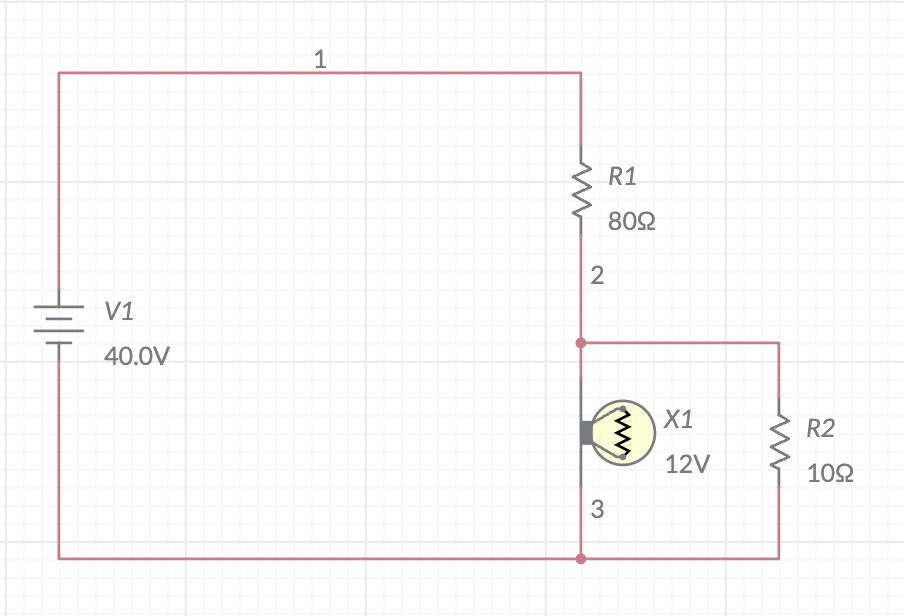
\includegraphics[keepaspectratio = true, width = 5in]{Q2(iv).png}
	\end{centering}
\end{figure}\\
It was observed that the brightness of X1 seems to decrease slightly as R2's resistance is decreased.\\
\\
As X1 and R2 are parallel, we use the following formula to calculate their combined resistance.\\
\[\frac{1}{R_T} = \frac{1}{R_1} + \frac{1}{R_2} + ... + \frac{1}{R_n}\]
\[\frac{1}{R_T} = \frac{1}{10} + \frac{1}{10} = \frac{1}{5}\]
\[R_T = 5\Omega \]\\
Now we can treat all of our components as if they are in series.\\
\[R_{Total} = R_1 + R_2 + ... + R_n\]
\[R_{Total} = 80 + 5 = 85\Omega\]\\
Using Ohm's Law, we can now find the current flowing through the circuit.\\
\[V = IR\]
\[40 = 85I\]
\[I = \frac{40}{85}A = \frac{8}{17} = 0.4371A\]\\
Using these values, we can now calculate the voltage drop after passing through each component.\\
\\
Starting with R1,\\
\[V_{R1} = I_{R1}R_{R1}\]
\[V_{R1} = \frac{8}{17} \times 80 = \frac{640}{17}V = 37.6471V\]\\
As X1 and R2 are parallel to each other, their voltages are equal.\\
We can calculate the voltage drop across X1 and R2 like so\\
\[V_{in} = V_{R1} + V_{R2}\]
\[40 = \frac{640}{17} + V_{R2}\]
\[V_{R2} = V_{X1} = 40 - \frac{640}{17} = 2.3529V\]\\
These calculations show that the bulb is dimmer because it has a lower input than in Q2(iii).\\
\\


\end{document}